\section{Initial Ideas}

While species analysis via IR detection relied upon phototransistors and optical filtering, radio signal detection introduces distinct challenges in circuit design and frequency testing. For our desired species – Gribbit and Zapple, our goal was to build a circuit capable of:

\begin{enumerate}
    \item Capturing AM-modulated radio signals.
    \item Selecting the correct carrier frequency (89kHz).
    \item Demodulating the signal to extract low-frequency data.
    \item Amplifying the signal to a detectable level.
\end{enumerate}

While the brief proposed using a tuned coil antenna, we opted for a standard inductor based on predictable characteristics and ease of integration. The table below compares both options:

\begin{table}[H]
    \centering
    \begin{tabular}{|l|l|l|}
        \hline
        \textbf{Inductor Type}     & \textbf{Tuned-Coil Antenna}    & \textbf{Standard Inductor} \\
        \hline
        Primary Role               & RF signal Reception            & Energy Storage             \\
        Ease of Use/Predictability & Requires Tuning                & No tuning required         \\
        Q Factor                   & High (Narrow Bandwidth)        & Moderate to High           \\
        Frequency Range            & Narrow                         & Broad                      \\
        Impedance Matching         & Must match RF system impedance & No need to match           \\
        Size                       & Larger                         & Compact                    \\
        Parasitic Effects          & High                           & Low                        \\
        \hline
    \end{tabular}
    \caption{Comparison of Inductor Types}
    \label{tab:inductors}
\end{table}

\section{Circuit Design}

The carrier frequency of 89kHz is isolated using a parallel LC resonant circuit. The resonance condition is given by the following formula:
\[
    f_0 = \frac{1}{2\pi\sqrt{RC}} \quad \rightarrow \quad LC = \frac{1}{(2\pi f_0)^2}
\]
For a \( f_0 = 89000\,\text{Hz} \), this gives:
\[
    LC \approx 3.2 \cdot 10^{-12}
\]

To achieve a narrower, more selective bandwidth, we require a higher quality factor which varies inversely with capacitance. We start with a 68pF capacitor, which implies the LC filter will require roughly 47mH of inductance to resonate at the carrier frequency. These values define the first stage of the filter circuit.
\begin{figure}[H]
    \centering
    \includegraphics[width=0.8\textwidth]{subpages/images/radio_LTspice_rc_circuit.png}
    \caption{RC Circuit in LTspice}
    \label{fig:rc_circuit}
\end{figure}

The LTspice simulation used an AC sweep to verify resonance. A sharp peak at ~89kHz confirmed accurate tuning and validated the LC component selection. However, in the grand scheme, the design revolves around a different source - the current was selected a simple means to analyse resonance.
\begin{figure}[H]
    \centering
    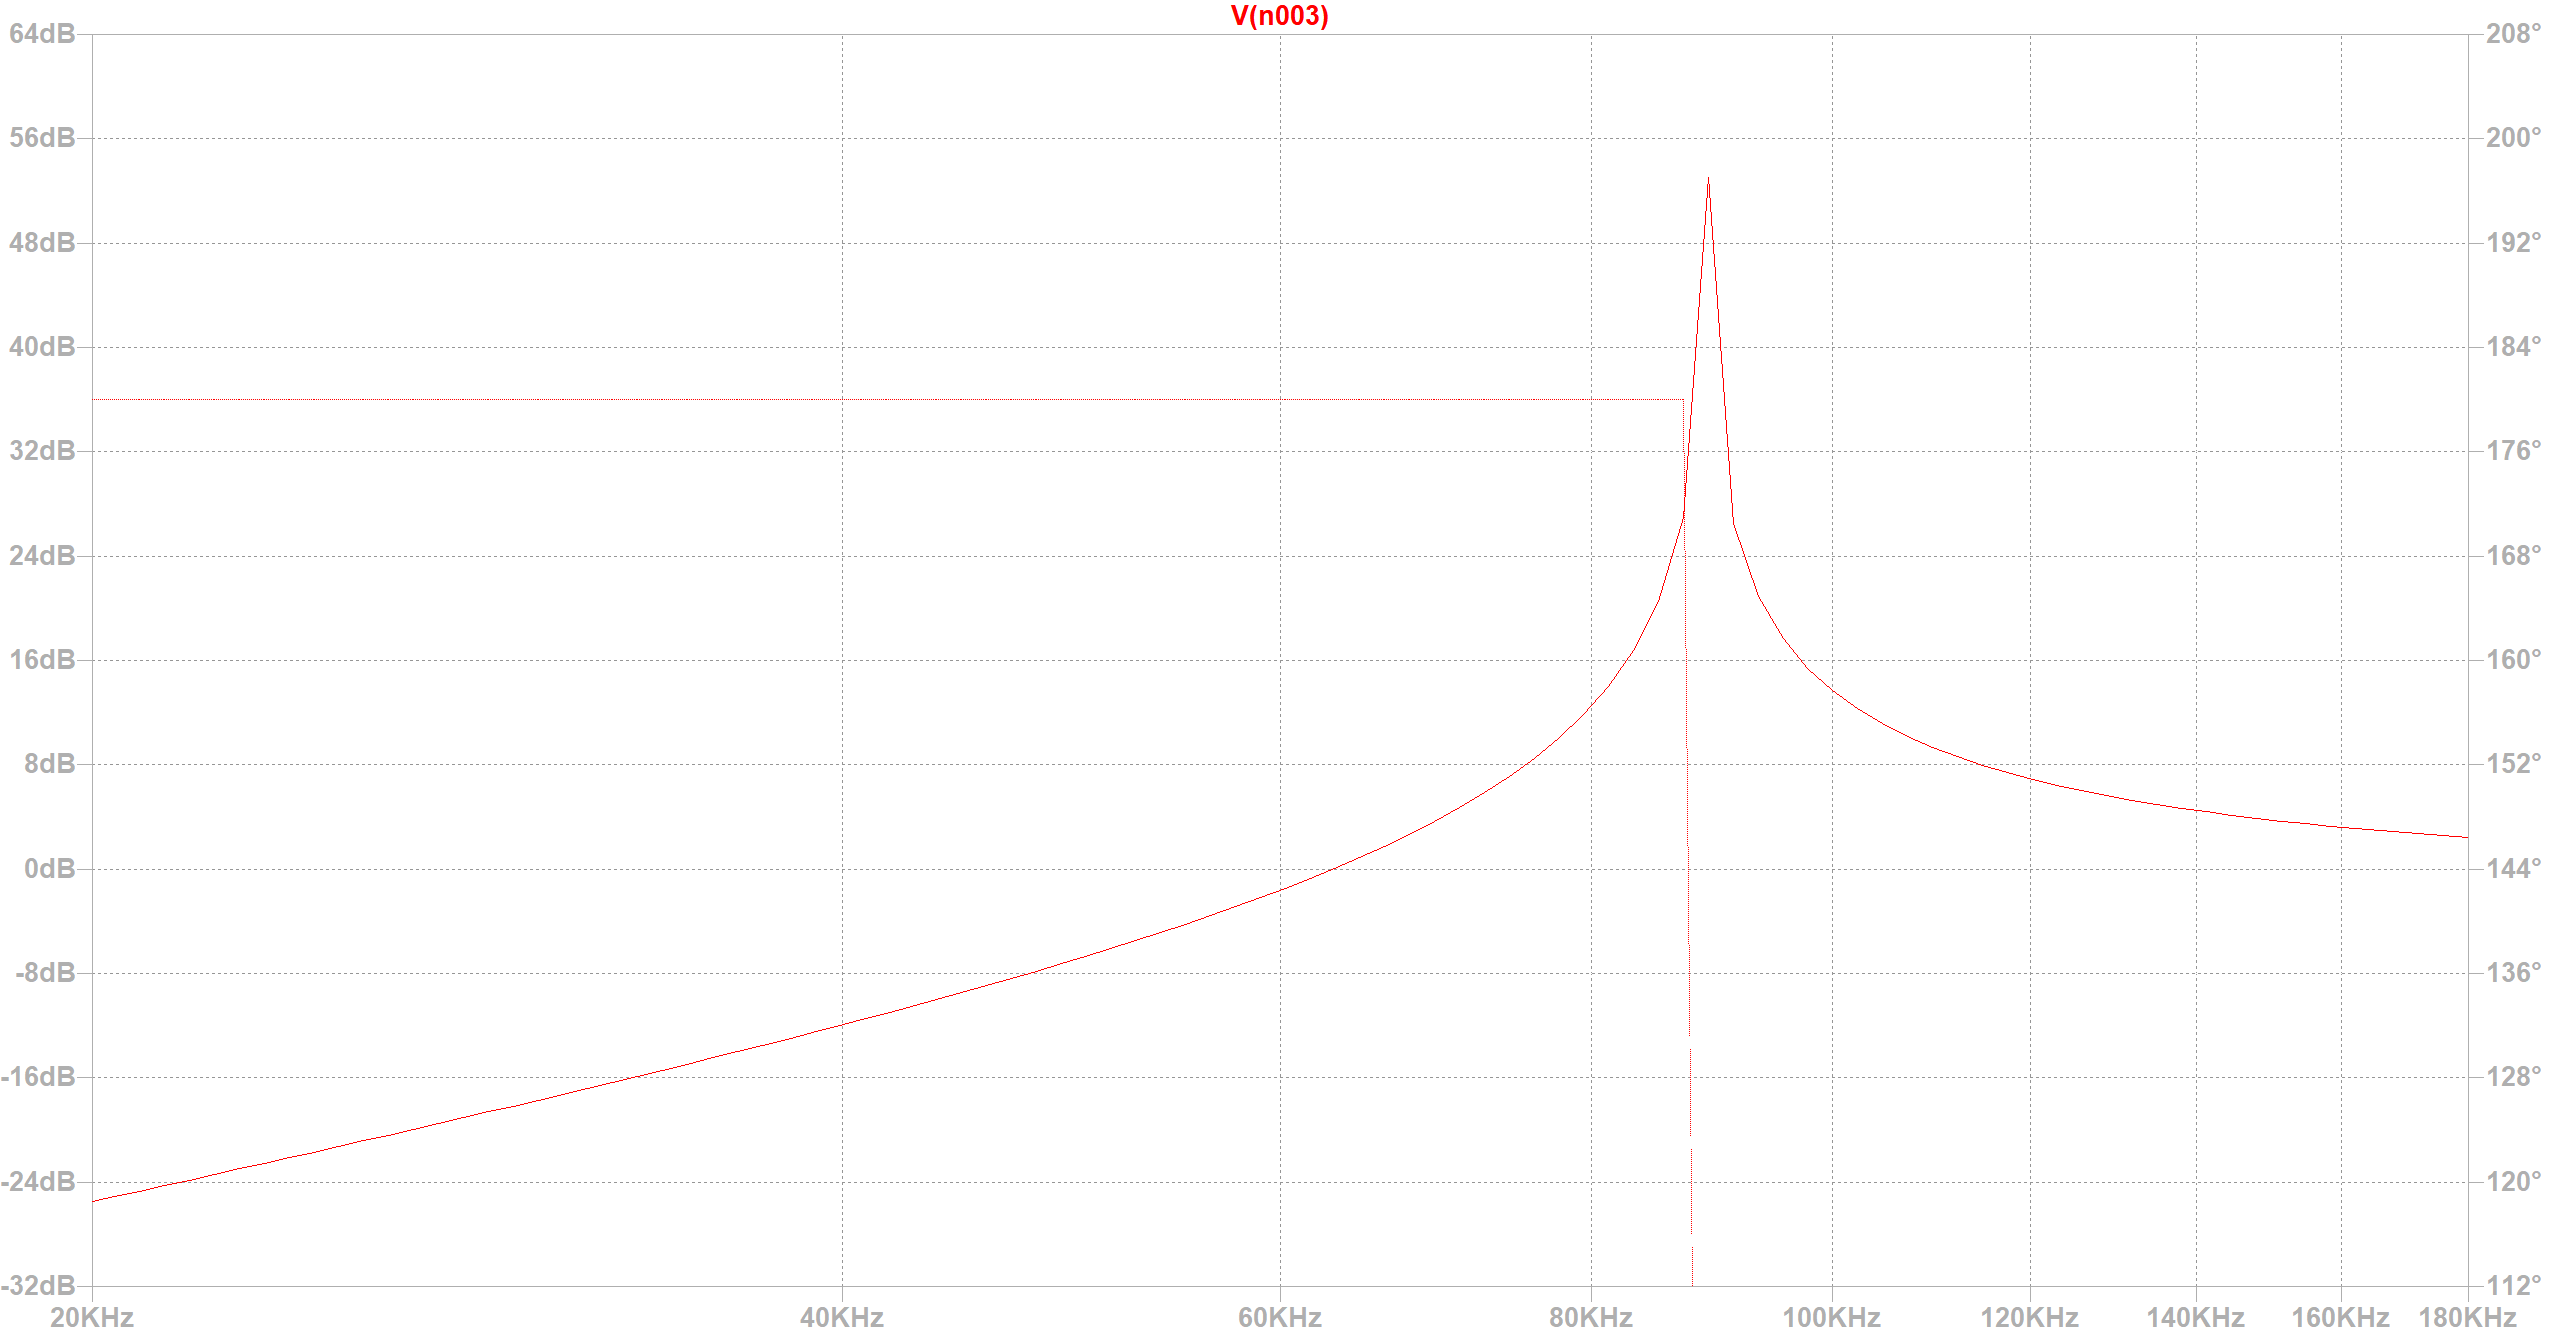
\includegraphics[width=0.8\textwidth]{subpages/images/radio_ac_waveform.png}
    \caption{AC Waveform Showing Resonance}
    \label{fig:ac_waveform}
\end{figure}

\subsubsection{Signal Modelling}

A behavioural voltage source: \( V=(1+0.5\cdot\sin(2\pi\cdot100\cdot\text{time})) \cdot \sin(2\pi\cdot89k\cdot\text{time}) \) was selected to simulate an actual received radio signal, for the following reasons:

\begin{itemize}
    \item The 89kHz carrier is represented by the outer sine function.
    \item The 100Hz message frequency, in the inner sine function, modulates the amplitude.
    \item The modulation depth ensures the signal swings between 0.5V and 1.5V, creating a clear envelope for detection.
\end{itemize}

\begin{figure}[H]
    \centering
    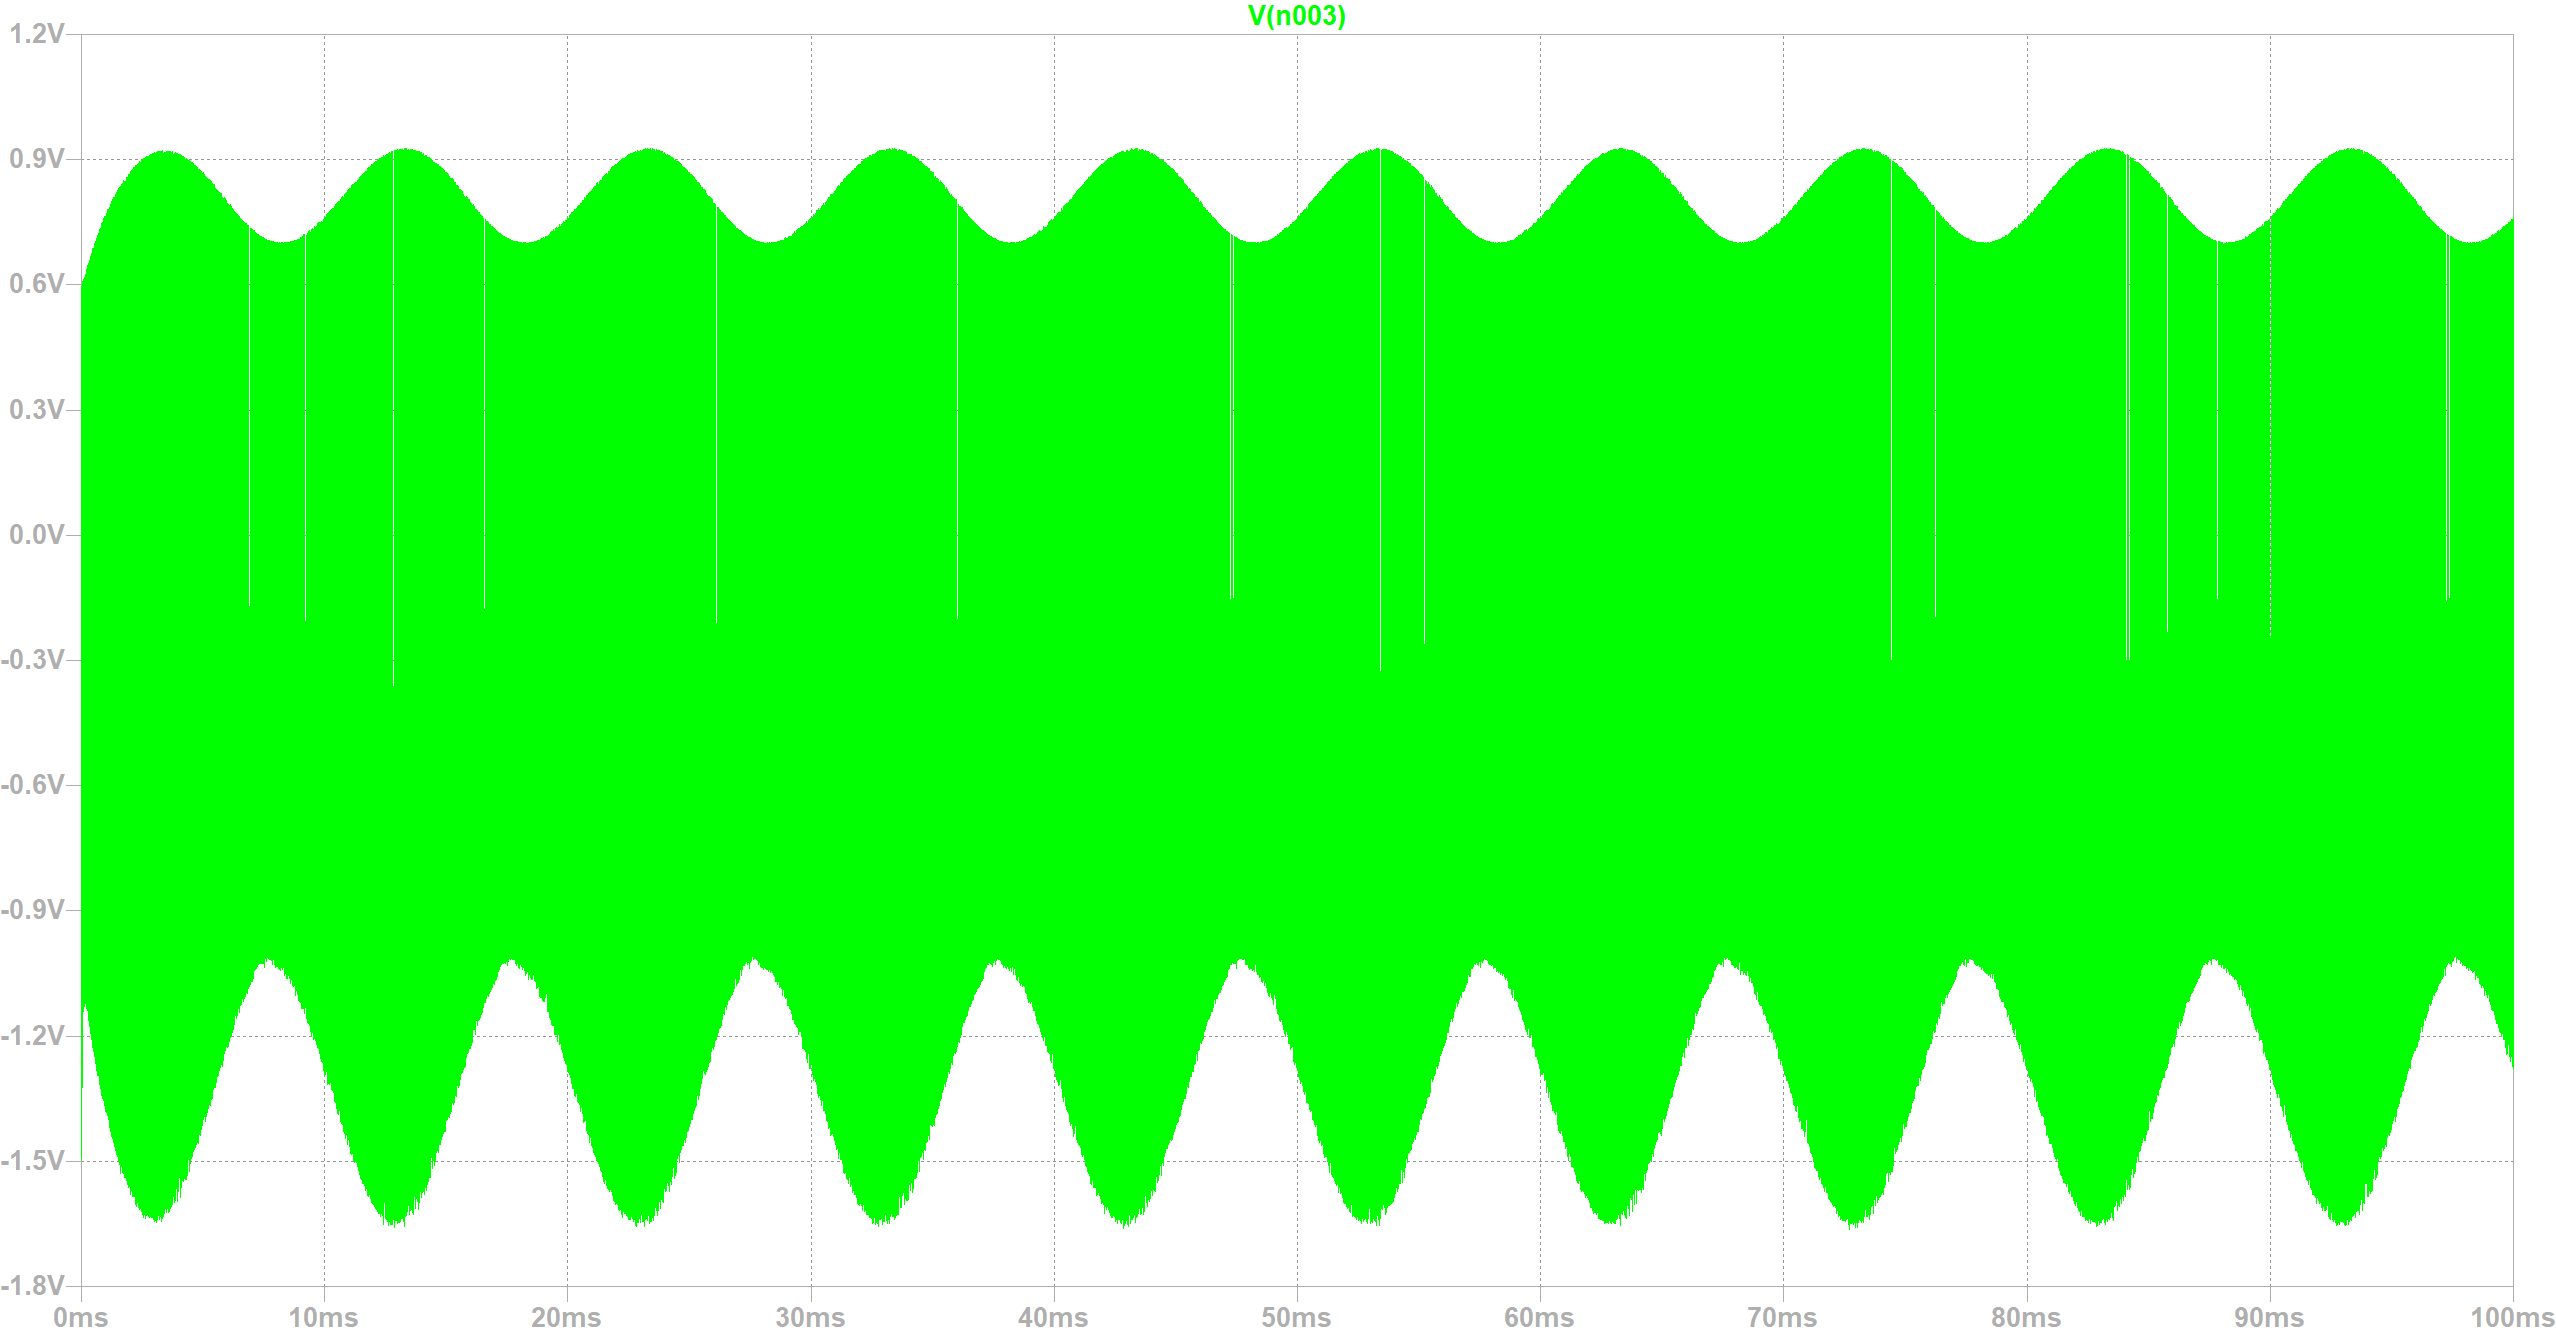
\includegraphics[width=0.8\textwidth]{subpages/images/radio_am_envelope_signal.png}
    \caption{An AM Envelope Signal}
    \label{fig:am_envelope}
\end{figure}

\subsubsection{Demodulation}

We now have the carrier frequency selected and now require the demodulation process using an envelope detector. Demodulation involves extracting a targeted information signal from a carrier signal once it has reached the receiver. Meanwhile, an envelope detector is a specific type of demodulator which serves the purpose of taking a high-frequency signal as input and extracting the varying amplitudes, which outputs the "outline" of the original amplitude modulation signal.

\begin{figure}[H]
    \centering
    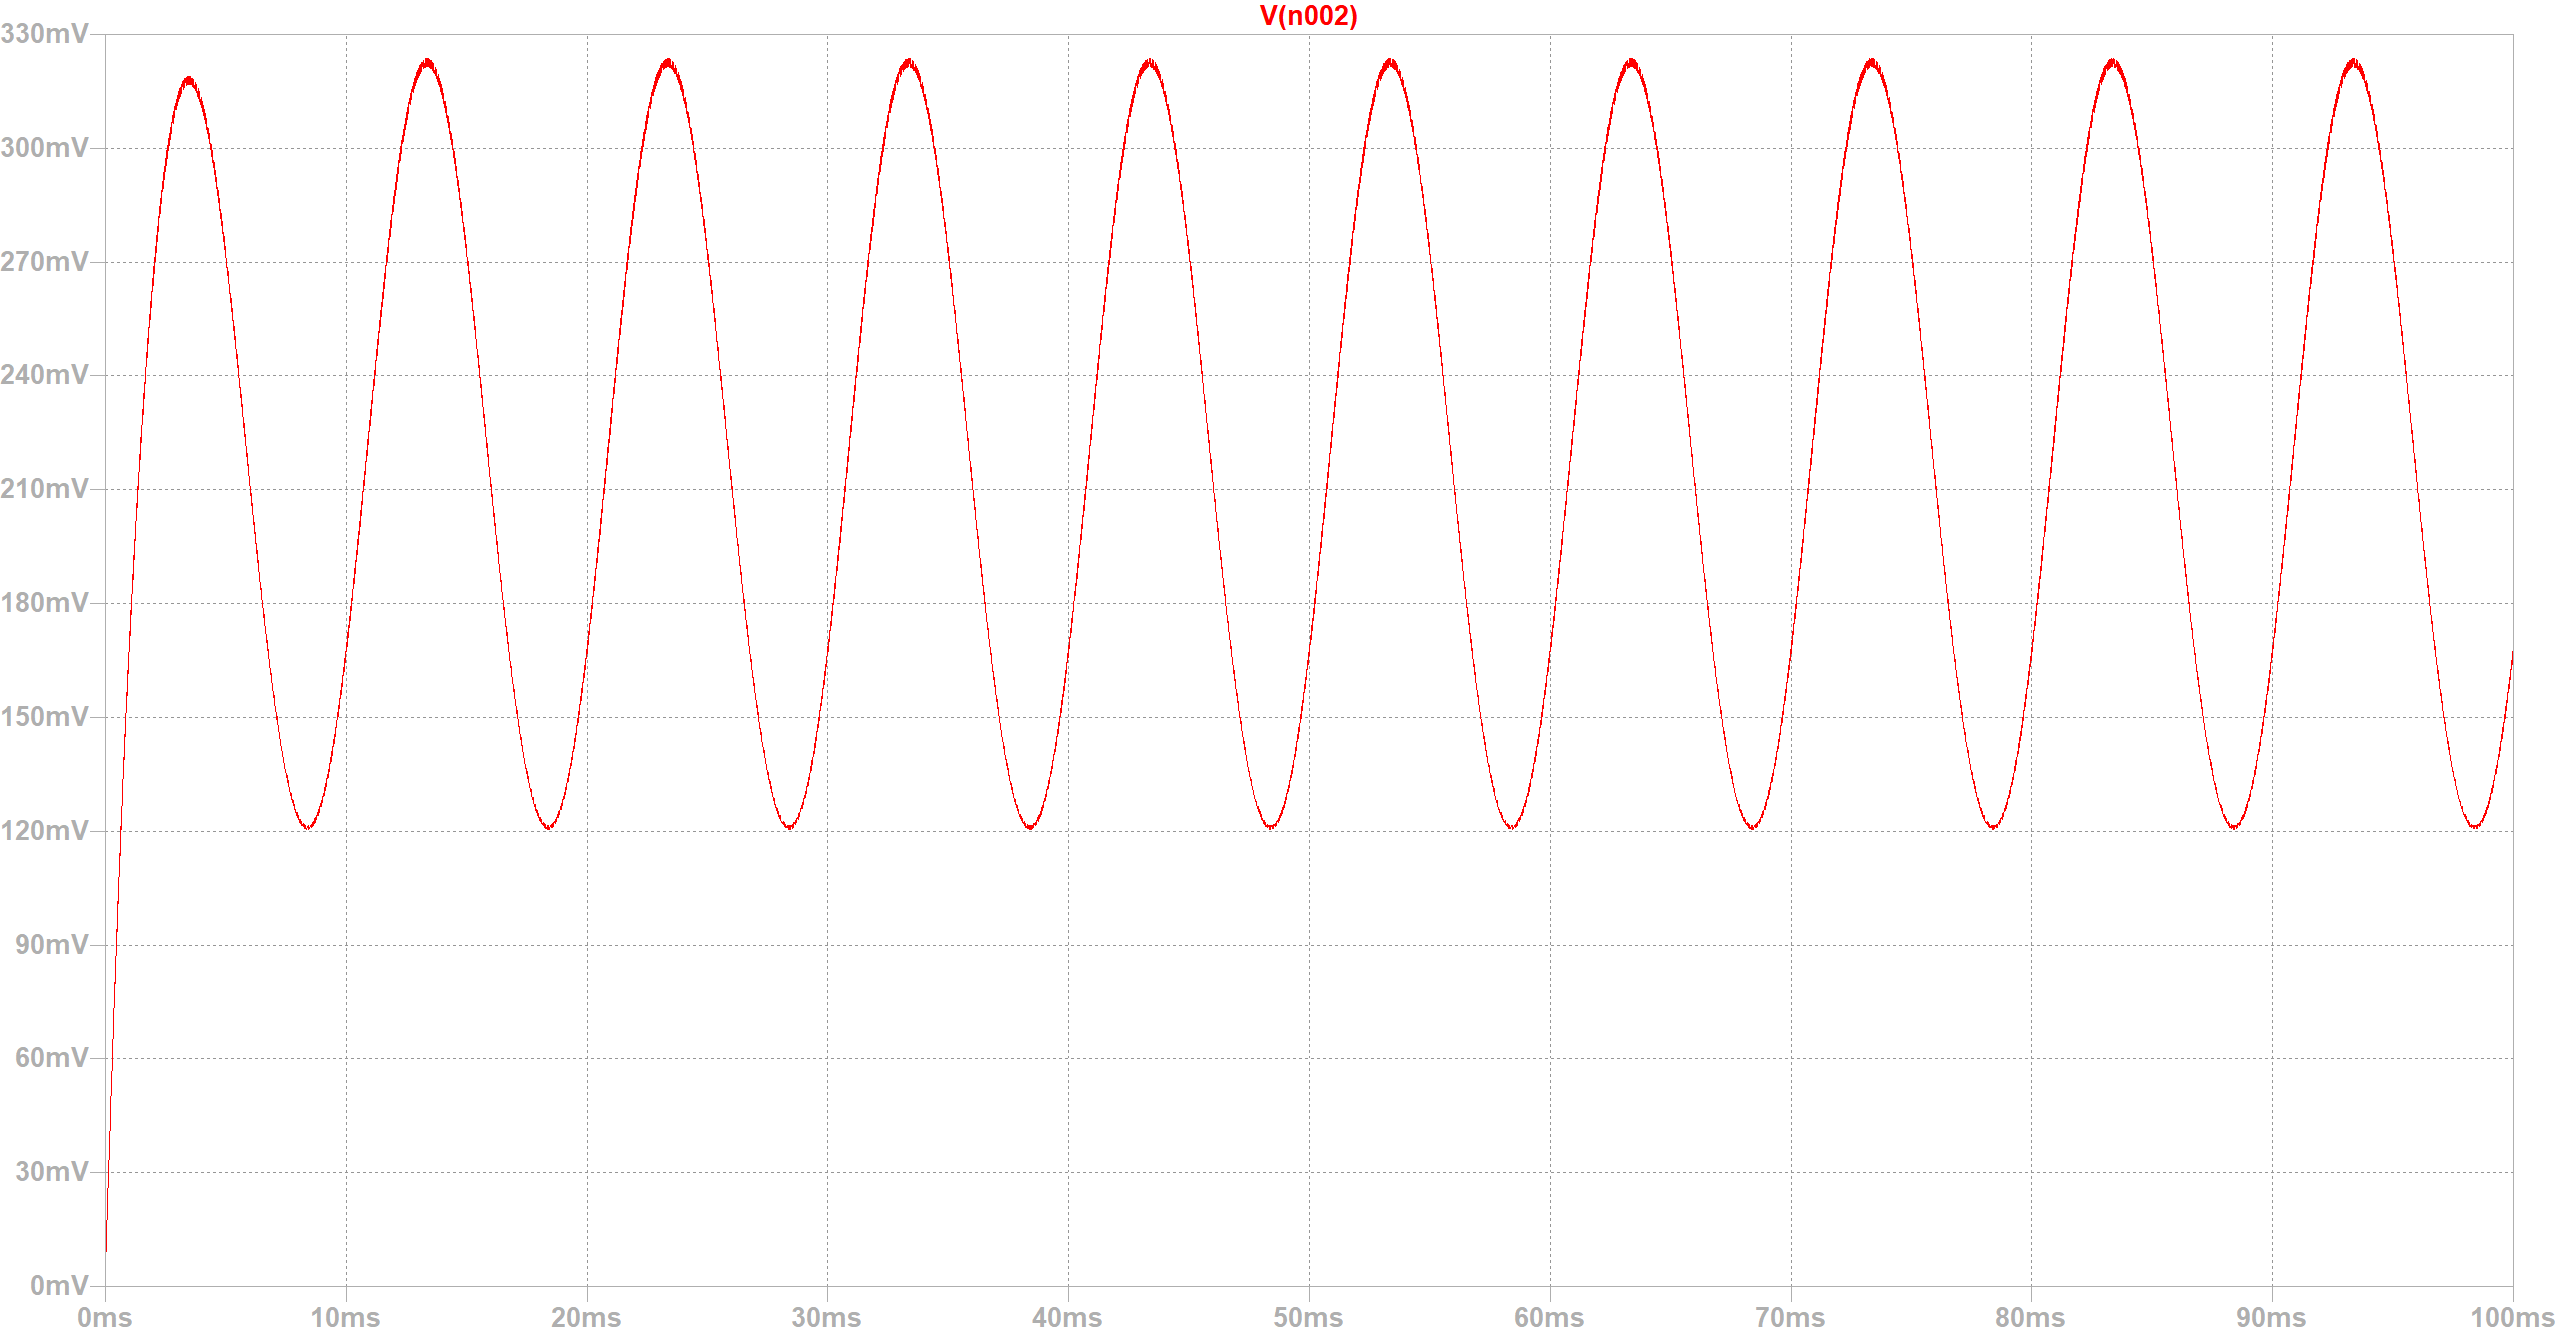
\includegraphics[width=0.8\textwidth]{subpages/images/radio_envelope_output.png}
    \caption{Output of the Envelope Detector }
    \label{fig:envelope_output}
\end{figure}

To extract the low-frequency data (e.g. 100Hz or 150Hz depending on species), the envelope detector was implemented using a diode, resistor, and capacitor:

\begin{itemize}
    \item The diode rectifies the signal.
    \item The RC filter smooths out the high-frequency carrier.
    \item The resulting waveform reflects the amplitude variation, i.e., the message signal.
\end{itemize}

This simulation output confirmed the demodulation stage successfully filtered out the carrier, leaving behind a readable low-frequency waveform.

\subsubsection{Signal Amplification}

Finally, the LTspice circuit concerns itself with amplifying the weak, raw signal stemming from the demodulation process. The envelope detector relies upon an imperfect diode which will trace out the desired waveform shape but fails to boost the power of the wave, rendering it faint for detection. Therefore, it was passed through a two-stage non-inverting op-amp amplifier. Each stage has a gain of:

\[
    1 + \frac{R_f}{R_{\text{in}}} = 1 + \frac{20k\Omega}{1k\Omega} = 21
\]

This leads to a total gain of \( 21 \cdot 21 = 441 \). We use two stages to avoid clipping or distortion from high single-stage gain, and bandwidth reduction or instability in the amplifier. A voltage follower precedes the amplifier to buffer the signal and ensure low output impedance from the envelope detector.

\subsubsection{Building and Testing}

The final circuit was built in stages, each validated independently:

\begin{enumerate}
    \item  Envelope Detection - verified with LTspice and matched our theoretical expectations. The diode and RC values didn't need tuning for a smooth envelope at 100-150Hz range as the theoretical values proved ample enough.
    \item Amplification - we first breadboarded and tested with synthetic input. The two-stage gain provided a clean, amplified waveform observable on an oscilloscope.
    \item Full System Integration - the final circuit captures the AM-modulated signal, filters and amplifies it for reliable species detection via \texttt{analogRead} in the Arduino code. It can distinguish between Gribbit (100Hz) and Zapple (150Hz) based on the output frequency. Refer to Chapter 8 for more detail on the code.
\end{enumerate}

\begin{figure}[H]
    \centering
    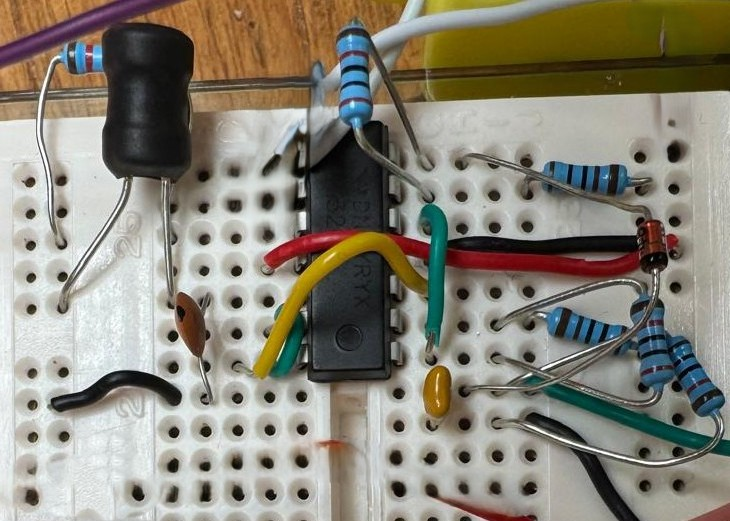
\includegraphics[width=0.8\textwidth]{subpages/images/radio_circuit.jpg}
    \caption{Final Built Circuit}
    \label{fig:radio_circuit}
\end{figure}

While our study on radio waves revealed the duck's frequencies through demodulation, this does not reveal the full picture. Beyond analysis of waves, there are polarities hidden which must be acknowledged. To ensure no duck is left unidentified, the focus now switches to the magnetic detection system.
